\documentclass[12pt]{scrartcl}
\usepackage[sexy]{james}
\usepackage[noend]{algpseudocode}
\setlength{\marginparwidth}{2cm}
\usepackage{answers}
\usepackage{array}
\usepackage{tikz}
\usepackage{graphicx}
\newenvironment{allintypewriter}{\ttfamily}{\par}
\usepackage{listings}
\usepackage{xcolor}
\usetikzlibrary{arrows.meta}
\usepackage{color}
\usepackage{mathtools}
\newcommand{\U}{\mathcal{U}}
\newcommand{\E}{\mathbb{E}}
\usetikzlibrary{arrows}
\Newassociation{hint}{hintitem}{all-hints}
\renewcommand{\solutionextension}{out}
\renewenvironment{hintitem}[1]{\item[\bfseries #1.]}{}
\renewcommand{\O}{\mathcal{O}}
\declaretheorem[style=thmbluebox,name={Chinese Remainder Theorem}]{CRT}
\renewcommand{\theCRT}{\Alph{CRT}}
\setlength\parindent{0pt}
\usepackage{sansmath}
\usepackage{pgfplots}

\usetikzlibrary{automata}
\usetikzlibrary{positioning}  %                 ...positioning nodes
\usetikzlibrary{arrows}       %                 ...customizing arrows
\newcommand{\eqdef}{=\vcentcolon}
\newcommand{\lint}{\int_{\overset{a}{\_}}^b}
\newcommand{\uint}{\int_a^{\bar{b}}}
\newcommand{\tr}{{\rm tr\ }}
\newcommand{\im}{{\rm Im\ }}
\newcommand{\spann}{{\rm span\ }}
\newcommand{\Col}{{\rm Col\ }}
\newcommand{\Row}{{\rm Row\ }}
\newcommand{\dint}{\displaystyle\int}
\newcommand{\dt}{\ {\rm d }t}
\newcommand{\PP}{\mathbb{P}}
\newcommand{\horizontal}{\par\noindent\rule{\textwidth}{0.4pt}}
\usepackage[top=3cm,left=3cm,right=3cm,bottom=3cm]{geometry}
\newcommand{\mref}[3][red]{\hypersetup{linkcolor=#1}\cref{#2}{#3}\hypersetup{linkcolor=blue}}%<<<changed

\tikzset{node distance=4.5cm, % Minimum distance between two nodes. Change if necessary.
         every state/.style={ % Sets the properties for each state
           semithick,
           fill=cyan!40},
         initial text={},     % No label on start arrow
         double distance=4pt, % Adjust appearance of accept states
         every edge/.style={  % Sets the properties for each transition
         draw,
           ->,>=stealth',     % Makes edges directed with bold arrowheads
           auto,
           semithick}}


% Start of document.
\newcommand{\sep}{\hspace*{.5em}}

\pgfplotsset{compat=1.18}
\begin{document}
\title{MATH410: Homework 7}
\author{James Zhang\thanks{Email: \mailto{jzhang72@terpmail.umd.edu}}}
\date{\today}

\definecolor{dkgreen}{rgb}{0,0.6,0}
\definecolor{gray}{rgb}{0.5,0.5,0.5}
\definecolor{mauve}{rgb}{0.58,0,0.82}

\lstset{frame=tb,
  language=Java,
  aboveskip=3mm,
  belowskip=3mm,
  showstringspaces=false,
  columns=flexible,
  basicstyle={\small\ttfamily},
  numbers=left,
  numberstyle=\tiny\color{gray},
  keywordstyle=\color{blue},
  commentstyle=\color{dkgreen},
  stringstyle=\color{mauve},
  breaklines=true,
  breakatwhitespace=true,
  tabsize=3
}

\maketitle

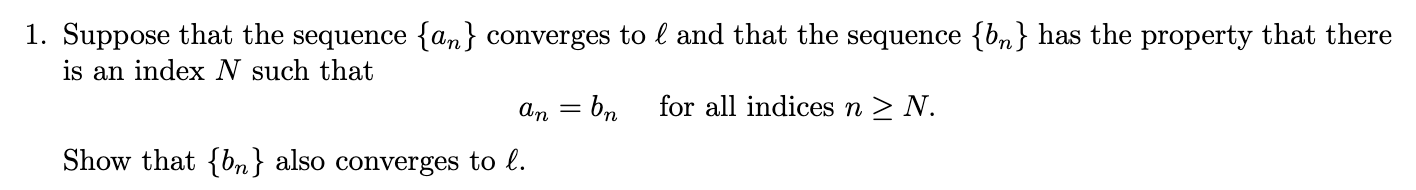
\includegraphics[width=14cm]{1.png}

\begin{proof}

\hfill

Let $P$ be a partition on $[a,b]$. By definition of Lower and Upper Integrals, $\lint f = \sup\{L(f, P) \ | \ \text{P partition on [a,b]}\}$
and $\uint f = \inf\{U(f, P) \ | \ \text{P partition on [a,b]}\}$.
First let us show that $\lint f \leq 0$. By definition of Darboux Lower Sum, 
\[\lint f = \sup\{\sum_{i=1}^n m_i (x_i - x_{i-1})\}\]
where $m_i := \inf\{f(x) \ | \ x \in [x_{i-1}, x_i]\}$. Recall that $\QQ$ and $\QQ^c$ are 
dense in each closed interval $[x_{i-1}, x_i]$. Thus, there exists some $x \in [x_{i-1}, x_i]$ such that 
$x \in \QQ \implies f(x) = 0$. Therefore, $m_i \leq 0 \ \forall \ i$. Since $x_i - x_{i-1} > 0$, then 
\[m_i(x_i - x_{i-1}) \leq 0 \ \forall \ i \implies \sum_{i=1}^n m_i(x_i - x_{i-1}) \leq 0 \ \forall \ \text{partitions}\] 
\[\implies \sup\{\sum m_i (x_i - x_{i-1}) \ | \ P \text{ partition on } [a,b]\} \leq 0 \implies \lint f\leq 0\]
Now we will show that $0 \leq \uint f$. 
\[\uint f = \inf\{\sum_{i=1}^n M_i(x_i - x_{i-1})\}\]
By density of $\QQ$ and $\QQ, \exists x \in [x_{i-1}, x_i]$ such that $f(x) = 0 \implies M_i = \sup\{f(x) \ | \ x \in [x_{i-1}, x_i]\}\geq 0 \ \forall \ i$. 
Therefore, 
\[M_i(x_i -x_{i-1}) \geq 0 \ \forall \ i \implies \uint f \geq 0\]
\[\lint f \leq 0 \leq \uint f\]
as desired.

\end{proof}

\newpage

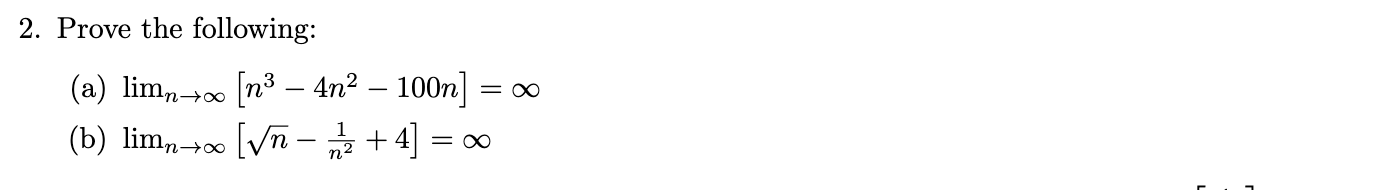
\includegraphics[width=14cm]{2.png}

\begin{proof}

\hfill

Let $P$ be a partition on $[a,b]$. First observe that
\[\lint f = \sup\{L(f, P) \ | \ \text{P partition on [a,b]}\}\]
and by substitution using the definition of Darboux Lower Sum, 
\[\lint f = \sup\{\sum_{i=1}^n m_i(x_i - x_{i-1}) \ | \ P \text{ partition on } [a,b]\}\]
where $m_i = \inf\{f(x) \ | \ x \in [x_{i-1}, x_i]\}$. Since $f(x) \geq 0 \ \forall \ x \in [a,b] \implies f(x) \geq 0 \ \forall \ x \in [x_{i-1}, x_i]$. 
Therefore, by definition of $\inf$ being the largest lower bound, $m_i \geq 0 \ \forall \ i$.
Since $x_i - x_{i-1} > 0$ by property of partition, $m_i(x_i - x_{i-1}) \geq 0 \ \forall \ i$ which implies that 
$\sum_{i=1}^n m_i(x_i - x_{i-1}) \geq 0$ for all partitions $P$. Thus,
\[\lint f \geq 0\]
as desired.

\end{proof}

\newpage

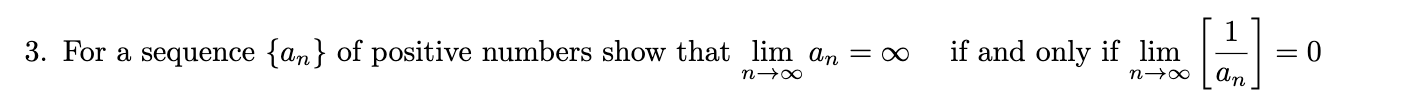
\includegraphics[width=14cm]{3.png}

\begin{proof}

\hfill

\begin{enumerate}[a.]

\item By definition of Darboux Lower Sums, we WTS that 
\[\sum_{i=1}^n m_i(x_i - x_{i-1}) \leq \sum_{i=1}^n p_i(x_i - x_{i-1})\]
or equivalently
\[\sum_{i=1}^n (p_i - m_i)(x_i - x_{i-1}) \geq 0\]
where $m_i := \inf\{g(x) \ | \ x \in [x_{i-1}, x]\}$ and $p_i := \inf\{f(x) \ | \ x \in [x_{i-1}, x_i]\}$.
Since $g(x) \leq f(x) \ \forall \ x \in [a,b] \implies g(x) \leq f(x) \ \forall \ x \in [x_{i-1}, x_i]$. Since $\inf$ is by definition 
the largest lower bound, intuitively $m_i \leq p_i \ \forall \ i \implies p_i - m_i \geq 0$. Since $x_i - x_{i-1} > 0$, 
then 
\[(p_i - m_i)(x_i - x_{i-1}) \geq 0 \ \forall \ i \implies \sum_{i=1}^n (p_i-m_i)(x_i - x_{i-1}) \geq 0 \]
\[\implies L(g, P) \leq L(f, P)\]

\item We WTS that $\lint g \leq \lint f$ or equivalently 
\[\sup\{L(g, P) \ | \ P \text{ partition on } [a,b]\} \leq \sup\{L(f, P) \ | \ P \text{ partition on } [a,b]\}\]
Assume on the contary that 
\[\sup\{L(g, P) \ | \ P \text{ partition on } [a,b]\} > \sup\{L(f, P) \ | \ P \text{ partition on } [a,b]\}\]
Then there must exist a partition $P^*$ such that 
\[L(g, P^*) > \sup\{L(f, P) \ | \ P \text{ partition on } [a,b]\}\]
However, from (a), recall that we showed that $L(g, P^*) \leq L(f, P^*)$
and so we've reached a contradiction. Therefore, 
\[\lint g \leq \lint f\]
\end{enumerate}

\end{proof}

\newpage

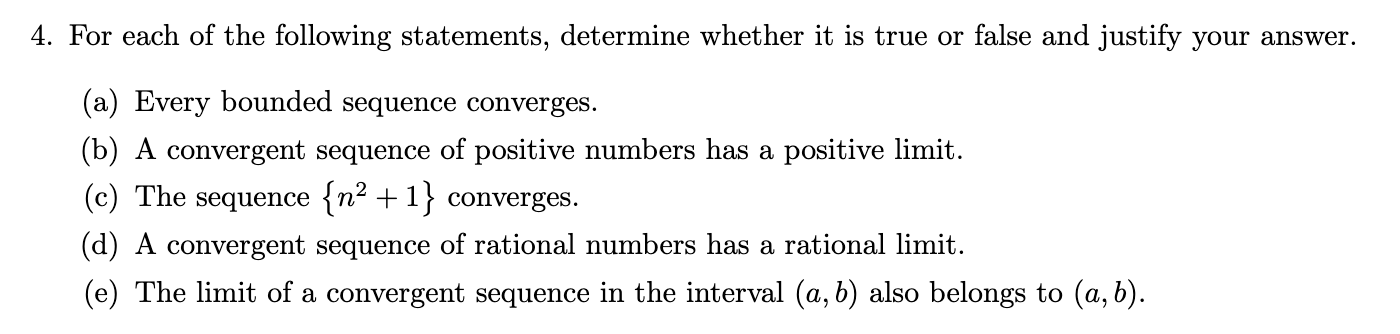
\includegraphics[width=14cm]{4.png}

\begin{proof}

\hfill

By definition of Darboux Lower and Upper Sums, we are given that 
\[\sum_{i=1}^n m_i(x_i - x_{i-1}) = \sum_{i=1}^n M_i(x_i - x_{i-1})\]
where $m_i$ is the inf and $M_i$ is the sup of the $ith$ subinterval. Rearranging above we can easily show that 
\[\sum_{i=1}^n (M_i - m_i)(x_i - x_{i-1}) = 0\]
Note that $x_i > x_{i-1} \ \forall \ 0$. Note that $m_i \leq M_i \ \forall \ i$ by properties of 
inf and sup. Note that $m_i = M_i \ \forall \ i$, otherwise, $L(f, P) < U(f, P)$ which contradicts a 
given. Therefore, for all closed subintervals $[x_{i-1}, x_i], m_i = M_i$. For any $f:[a,b] \to \RR$, 
if $\inf(f) = \sup(f) = c, c \in \RR$ then $f(x) = c \ \forall \ x \in [a,b]$. Suppose on the contrary there existed an 
$x_0 \in [a,b]$ such that $f(x) > c$. Then $c$ is not the sup. Similar for the other direction. Thereefore, for 
any closed interval, if the inf and sup are equal, then all functional values on the closed intervals are a constant.

\hfill

Note that subintervals are connected and that for any $x_i, x_i \in [x_{i-1}, x_i]$ and $x_i \in [x_i, x_{i+1}]$.
Suppose we have two connected subintervals such that 
 $f(x) = c \ \forall \ x \in [x_{i-1}, x_i]$ and $f(x) = d \ \forall \ x \in [x_i, x_{i+1}], c, d \in \RR$.
Note that $f(x_i) = c = d \implies f(x) = a \ \forall \ x \in [x_{i-1}, x_{i+1}]$. Repeating this process 
for all guaranteed connected subintervals in the partition yields that $f(x) = c \ \forall \ x \in [a, b]$. 

\end{proof}

\newpage

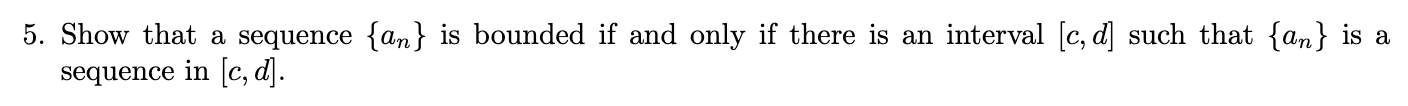
\includegraphics[width=14cm]{5.png}

\begin{proof}

\hfill

\begin{enumerate}[a.]

\item First let us show that $\int_a^b x \ dx$ is integrable. By the Archimedes-Riemann Theorem, an $f$
that is bounded is integrable if $\ \exists \ \{P_n\}$ such that 
\[\lim_{n\to\infty}((U(f, P_n) - L(f, P_n))) = 0\]
Let $P_n$ be the regular partition such that all subintervals are the same length
\[P_n = \{a, a + \frac{b-a}{n}, a + 2\frac{b-a}{n}, \ldots, b\} \implies x_i = a + i\frac{b-a}{n}\]
Therefore, 
\[\lim_{n\to\infty}(U(f, P_n) - L(f, P_n)) = \lim_{n\to\infty} \sum_{i=1}^n (M_i - m_i)(x_i - x_{i-1})\]
\[= \lim_{n\to\infty}\sum_{i=1}^n (a + i\frac{b-a}{n} - a - (i-1)\frac{b-a}{n})(\frac{b-a}{n}) = \lim_{n\to\infty}(b-a)^2 \sum_{i=1}^n \frac{1}{n^2}\]
\[= \lim_{n\to\infty}\frac{b-a}{n} = 0\]
Therefore, $f(x) = x$ is integrable and by the "moreover" part of the AR Theorem
\[\int_a^b x = \lim_{n\to\infty}U(f, P_n) = \lim_{n\to\infty}\sum_{i=1}^n (a + i\frac{b-a}{n})(\frac{b-a}{n})\]
\[= \lim_{n\to\infty}\frac{b-a}{n}(\sum_{i=1}^n a + \frac{b-a}{n}\sum_{i=1}^n i) = \lim_{n\to\infty}\frac{b-a}{n} (an + \frac{(b-a)(n+1)}{2})\]
\[= ab-a^2 + \lim_{n\to\infty}\frac{(b-a)^2(n+1)}{2n} = ab - a^2 + \lim_{n\to\infty}\frac{(b^2 - 2ab + a^2)(n+1)}{2n}\]
\[ = ab - a^2 + \frac{b^2 - 2ab + a^2}{2} = \frac{b^2 - a^2}{2}\]
as desired.

\item Let us show that $f(x) = 4x + 1$ is integrable. Let $P_n$ be a regular partition such that 
\[P_n = \{0, \frac{1}{n}, \frac{2}{n}, \ldots, 1\} \implies x_i = \frac{i}{n}\]
Observe that 
\[\lim_{n\to\infty}(U(f, P_n) - L(f, P_n)) = \lim_{n\to\infty}\sum_{i=1}^n (M_i - m_i)\frac{1}{n}\]
Note that the sup and inf are $M_i = \frac{4i}{n} + 1$ and $m_i = \frac{4(i-1)}{n} + 1 \implies M_i - m_i = \frac{4}{n}$.
Thus, 
\[\lim_{n\to\infty}(U(f, P_n) - L(f, P_n)) = \lim_{n\to\infty}\sum_{i=1}^n \frac{4}{n^2} = \lim_{n\to\infty}\frac{4}{n} = 0\]
which means $f$ is integrable and by the AR theorem
\[\int_0^1 4x + 1 dx = \lim_{n\to\infty}U(f, P_n) = \lim_{n\to\infty}\sum_{i=1}^n (\frac{4i}{n} + 1)(\frac{1}{n})\]
\[= \lim_{n\to\infty}\sum_{i=1}^n \frac{4i}{n^2} + \frac{1}{n} = \lim_{n\to\infty}\frac{4n(n+1)}{2n^2} + 1 = 3\]

\item First let us show that $f(x) = x^2$ is integrable. Let $P_n$ be the regular partition once more 
such that 
\[P_n = \{a, a + \frac{b-a}{n}, a + 2\frac{b-a}{n}, \ldots, b\} \implies x_i = a + i\frac{b-a}{n}\]
\[\lim_{n\to\infty}(U(f, P_n) - L(f, P_n)) = \lim_{n\to\infty} \sum_{i=1}^n (M_i - m_i)(x_i - x_{i-1})\]
\[ = \lim_{n\to\infty}\sum_{i=1}^n (M_i - m_i)(\frac{b-a}{n})\]
Now observe that $M_i = (a + i\frac{b-a}{n})^2$ and $m_i = (a + i\frac{b-a}{n} - \frac{b-a}{n})^2$
and this limit can be shown to approach to 0.
Furthermore, 
\[\int_a^b = \lim_{n\to\infty}U(f, P_n) = \lim_{n\to\infty} \sum_{i=1}^\infty (a + i\frac{b-a}{n})^2(\frac{b-a}{n})\]
\[= \frac{b^3-a^3}{3}\]

\end{enumerate}

\end{proof}

\newpage

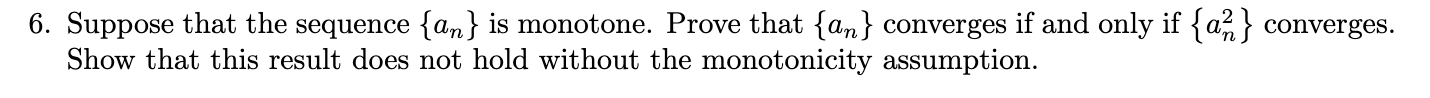
\includegraphics[width=14cm]{6.png}

\begin{proof}

\hfill

Since $f, g$ are integrable, there exists two Asop $P_n$ and $Q_n$ such that 
\[\lim_{n\to\infty}(U(f, P_n) - L(f, P_n)) = 0 \text{ and } \lim_{n\to\infty}(U(g, Q_n) - L(g, Q_n)) = 0\]
Now let us define a new sequence $R_n$ that is a refinement of $P_n$ and $Q_n$. Therefore, 
by the Refinement Lemma, 
\[L(f, P_n) \leq L(f, R_n) \text{ and } U(f, R_n) \leq U(f, P_n)\]
\[L(g, Q_n) \leq L(g, R_n) \text{ and } U(g, R_n) \leq U(Q, P_n)\]
Combining some of the above inequalities, note that 
\[U(f, R_n) - L(f, R_n) \leq U(f, P_n) - L(f, P_n)\]
\[U(g, R_n) - L(g, R_n) \leq U(g, Q_n) - L(g, Q_n)\]
Note that both right hand sides converge to 0 because $f$ and $g$ are integrable. Therefore, 
by the Comparison Lemma, the left hand sides also converge to 0, which means
$R_n$ is an Asop for both $f$ and $g$ on $[a,b]$.

\end{proof}

\newpage

\end{document}

